% !TeX spellcheck = en_US
\section{Ranking window}\label{section:ranking}

In this section ranking window is described. Ranking data is stored in .ranking file. You can open this file by double clicking on it in workspace tree.

Ranking is created by chosen ranking method, with exploits preference graph. Created ranking is a solution to ranking problem.

\begin{figure*}[!ht] 
	\centering
	\makebox[\textwidth]{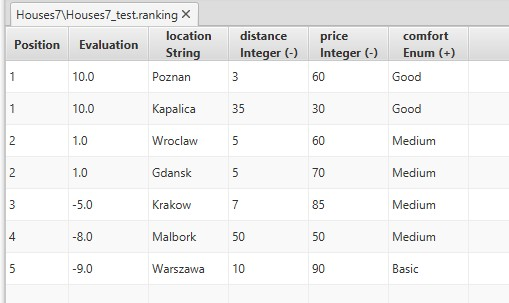
\includegraphics[width=.6\paperwidth]{raw/ranking}}
	\caption{Ranking for Houses7}
\end{figure*}

Each row in table represents position of object in ranking. Also objects attributes are displayed as additional columns. Columns for attributes contains field type and cost/gain criterion indicator. If you hover over column header, tooltip will be displayed with additional information.

Columns can be reordered and are sortable. This is not saved to file, because this files are read only. You can also export selected rows to CSV format. You can do this by selecting rows and choosing ''Copy selected rows'' option from context menu. Columns names will be used for CSV header.

\vfill\newpage